% ==============================================================================
% POSTER STYLE DON'T MODIFY
\documentclass[final]{beamer}
\setbeamertemplate{caption}[numbered]
\beamertemplatenavigationsymbolsempty

\usepackage[orientation=portrait,size=a0,scale=1.25]{beamerposter}
\usepackage[utf8]{inputenc}
\usepackage[T1]{fontenc}
\usepackage{tikz}
\usepackage{lmodern}
\usepackage{amsmath,amsthm, amssymb, latexsym}
\usepackage{url}
\usepackage{ragged2e}
\usepackage{parskip}

\usepackage{algpseudocode}
\usepackage{algorithm}
\MakeRobust{\Call}

\usepackage{multicol}
\setlength{\columnsep}{80pt}

\usepackage{graphicx}
\usepackage{listings}

% used for drawing section lines etc...
\usepackage{tikz}
\tikzset{every mark/.append style={scale=3.5}}
\usepackage{pgfplots}
\usepackage{pgfplotstable}
\pgfplotsset{	
	compat=newest,
	width=7.5in,
	max space between ticks=100pt,
	every axis plot post/.append style={ultra thick},
	/pgfplots/ylabel absolute/.style={%
		/pgfplots/every axis y label/.style={at={(0,0.5)},xshift=4em,rotate=90},
		%/pgfplots/every y tick scale label/.style={
		%at={(0,1)},above right,inner sep=0pt,yshift=0.3em
		%},
	},
}

\linespread{1.05}
\geometry{hmargin=2.5cm}

% define basic colors
\definecolor{black}  {RGB}{0,0,0} 		%%% text color
\definecolor{blue}  {RGB}{20,66,129} 		%%% title and subsection color
\definecolor{lightblue}  {RGB}{28,130,185} 	%%% section color
\definecolor{lightgrey}  {RGB}{255,253,250} 	%%% background color

\setbeamercolor{structure}{fg=blue}
\setbeamercolor{colorbar}{fg=black,bg=blue}
\setbeamercolor{normal text}{fg=black}
\beamertemplatesolidbackgroundcolor{lightgrey}

%set bibliography style
\setbeamertemplate{bibliography item}[text]
\setbeamercolor{bibliography item}{fg=black,bg=lightgrey}
\setbeamercolor{bibliography entry author}{fg=black,bg=lightgrey}
\setbeamerfont{bibliography item}{size=\small}
\setbeamerfont{bibliography entry author}{size=\small}

% poster title
\setbeamertemplate{headline}{
  \leavevmode
  \vskip 2cm
  \begin{columns}
    \begin{column}{0.15\linewidth}
      \begin{center}
        %\includegraphics[width=0.55\linewidth]{logo}
      \end{center}
    \end{column}
    
    \begin{column}{.7\linewidth}
      \centering{
        {\color{lightblue}
        \setlength\lineskip{20pt}
        \textbf{\huge{\inserttitle}}\\[1ex]}
      	\vskip 1cm
        {\color{fg} \Large{\insertauthor}\\[1ex]}
        {\color{fg} \large{\insertinstitute}\\[1ex]}
      }
      \vskip 1cm
    \end{column}
    
    \begin{column}{.15\linewidth}
      \begin{center}
        %\includegraphics[width=\linewidth]{eda-logo}
      \end{center}
    \end{column}

    %%%\vspace{5cm}
  \end{columns}
}

% poster foot
\setbeamertemplate{footline}{
  \leavevmode
  %\vskip 1cm
  
  % horizontal line
  \begin{flushleft}
    \begin{tikzpicture}[remember picture,overlay]
      \shade [inner color=lightblue,outer color=lightgrey] (0,0) rectangle (\textwidth,0.3cm);
    \end{tikzpicture}
  \end{flushleft}
        
  \vskip 1cm
        
  \begin{center}
    \begin{columns}[c]
	  \begin{column}{0.1\linewidth}
	    \begin{center}
	      %\includegraphics[width=6cm]{rma_1600.png}
	    \end{center}
	  \end{column}
	    
	  \begin{column}{.4\linewidth}
	    \begin{center}
	      %\includegraphics[width=6cm]{EURECOM_logo_quadri.pdf}
          \color{lightblue}
          \setlength\lineskip{20pt}
          \textbf{\Large{Cyber Defence Lab\\}}
          \large{Royal Military Academy\\
          \url{www.cylab.be}}
	    \end{center}
	  \end{column}
	    
	  \begin{column}{.1\linewidth}
	    \begin{center}
           %\includegraphics[width=6cm]{symantec-logo-300dpi.png}
	    \end{center}
      \end{column}
    \end{columns}
  \end{center}
  
  \vskip 1cm
}

% Section
\renewcommand{\section}[1]{
    % horizontal line
    %\par\vskip\medskipamount%
    %\begin{flushleft}
    \begin{tikzpicture}[remember picture,overlay]
      \shade [inner color=lightblue,outer color=lightgrey] (0,0) rectangle (\columnwidth,0.3cm);
    \end{tikzpicture}
    %\end{flushleft}
    
    \vskip 1.25cm

    \begin{center}
      %\vskip1cm
      \textcolor{lightblue}{\textbf{\Large #1}}
      %\parskip0pt\par
    \end{center}

    %\begin{flushleft}
    \vskip 0.25cm
    
    % horizontal line
    \begin{tikzpicture}[remember picture,overlay]
      \shade [inner color=lightblue,outer color=lightgrey] (0,0) rectangle (\columnwidth,0.3cm);
    \end{tikzpicture}
    %\end{flushleft}
    
    \parskip 10pt \par
    \justifying
}

%%% Sub-section
\renewcommand{\subsection}[1]{
  %\par\vskip\medskipamount%
  %\begin{center}
  \vskip 1.2cm
  \textcolor{lightblue}{\textbf{\textsl{\large #1}}}
  %{\parskip0pt\par}
  %\end{center}
  \justifying
}

% ==============================================================================
% Title, date and authors of the poster
\title{Smart Router}

\author[shortname]{
	Thibault Debatty \inst{1} \and
	Pietro Michiardi \inst{2} \and
	Olivier Thonnard \inst{3} \and
	Wim Mees \inst{1}
}
\institute[shortinst]{
	\inst{1} Royal Military Academy, Brussels, Belgium \and
  \inst{2} EURECOM, Campus SophiaTech, France \and
  \inst{3} Symantec Research Labs, Sophia Antipolis, France
}



% ==============================================================================
% Content of the poster

\usebackgroundtemplate{%
\tikz\node[opacity=0.1] {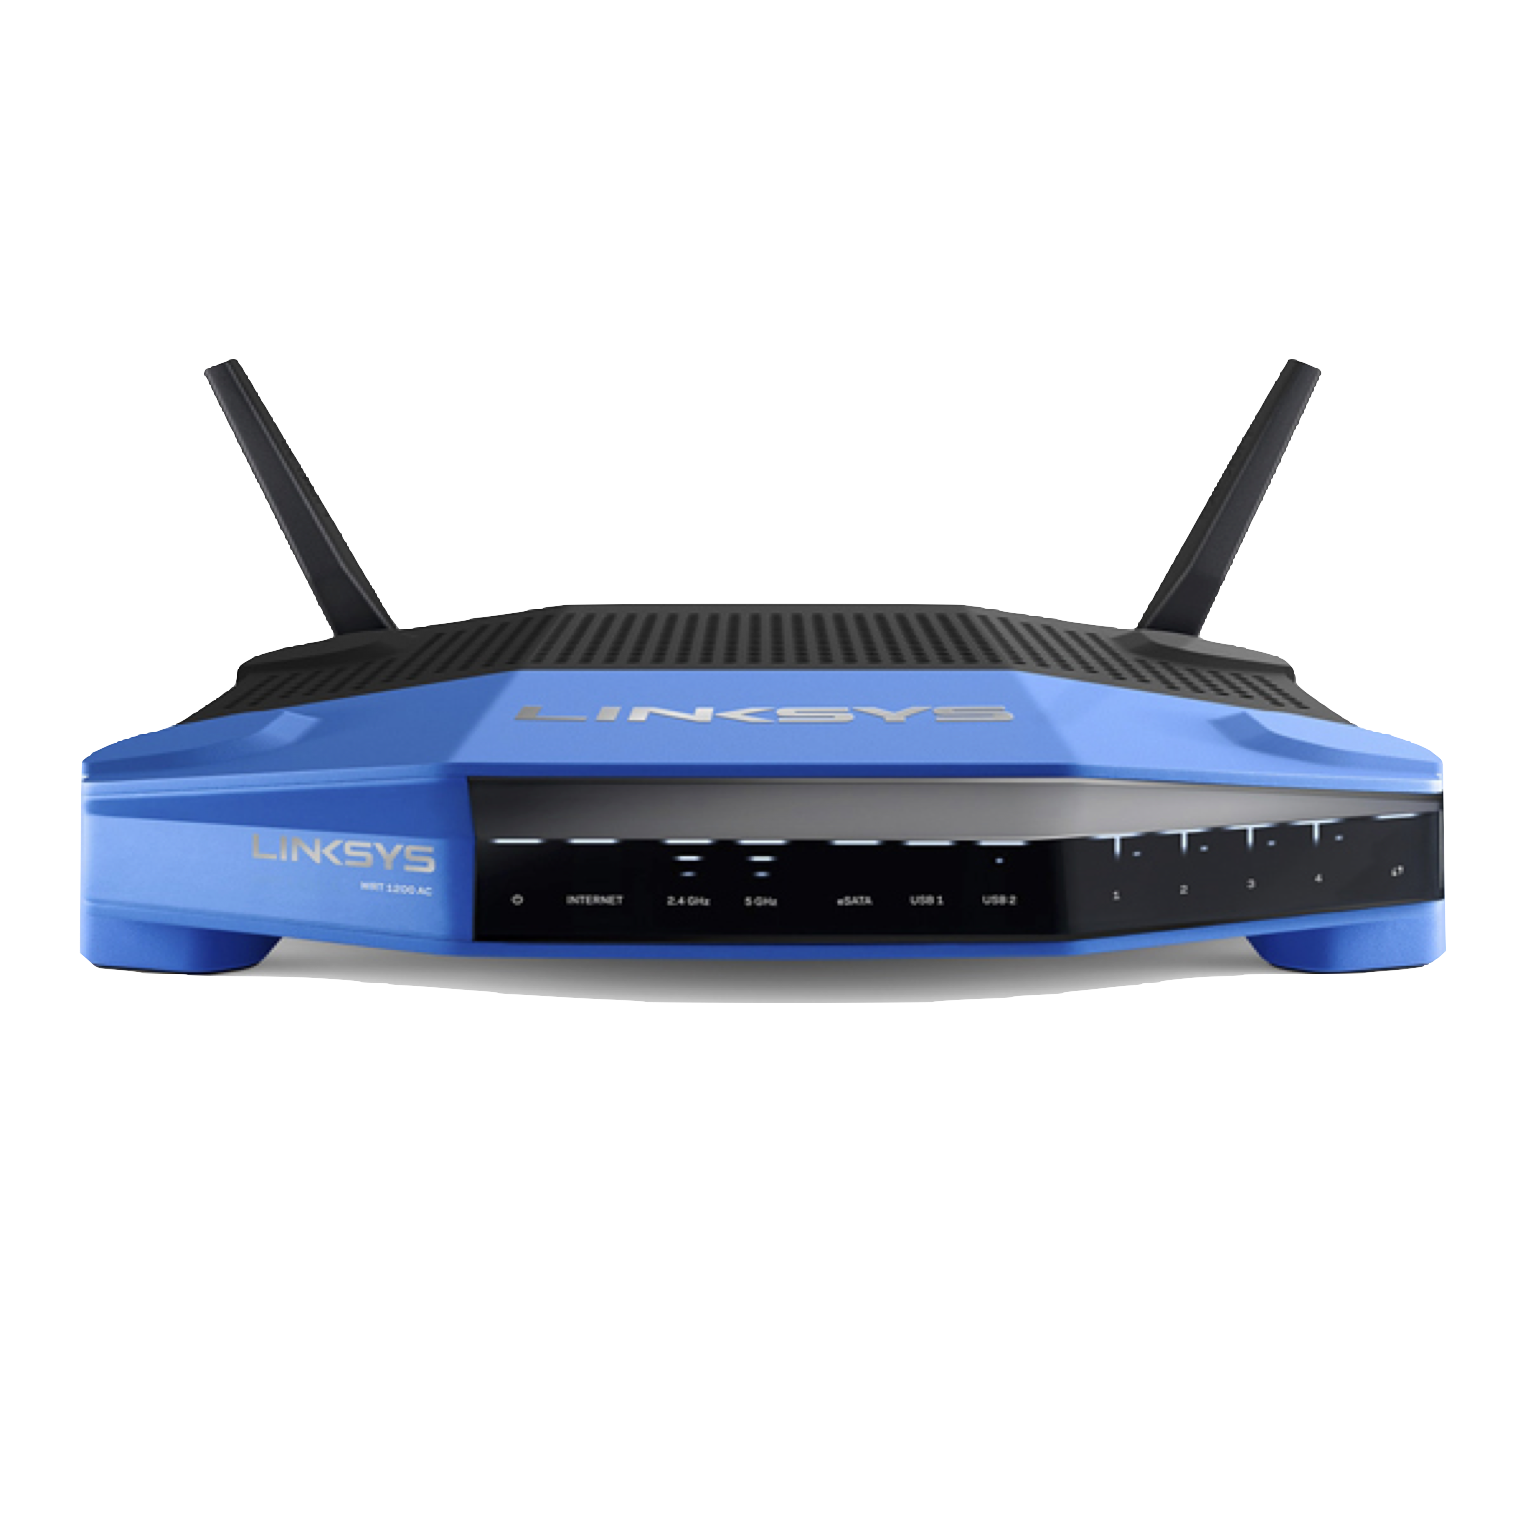
\includegraphics[height=\paperheight,width=\paperwidth]{Pictures/wrt1200ac.png}};}




\begin{document}
\begin{frame}{}
\begin{multicols}{3}



\section{Introduction}
The number of IoTs devices present in our houses is constantly growing up. Smart-TVs, smart-lights,IP-cameras and number others are all connected to the Internet to be managed from outside our homes. But how can we, in as SOHO context, monitor these devices to be sure they only do the work they should. So how to be sure they are not botnets ? 

\subsection{Goal}\\
The goal of this project is to monitor IoT traffic of a SOHO (Small Office, Home Office) network. By sniffing and analyzing it, this project can send alerts when an IoT has an unusual network traffic. For example, if it suddenly begins to send random request to random IP addresses around the world.

Only IoT traffic is interesting for this type of project because Iot devices only go to the same servers. Devices like laptops are used for example to surf the web and then it is never the same destinations. So sniffing non-IoT traffic is not the goal of this project. 



\section{Architecture}

The smart router is designed to be installed between the connected devices and the Internet, such that it can intercept and analyze the traffic generated by the devices. It is composed of 3 main modules:

\begin{itemize}
\item Traffic sniffer,
\item Traffic analyzer,
\item Web interface
\end{itemize}
%This project was initially designed from Ubuntu machine but was then adapted to work on an OpenWRT distribution which is more adapted from network embedded devices. This project was developed in Python3.

%\subsection{Design}\\ 


%The design of the router is the next one

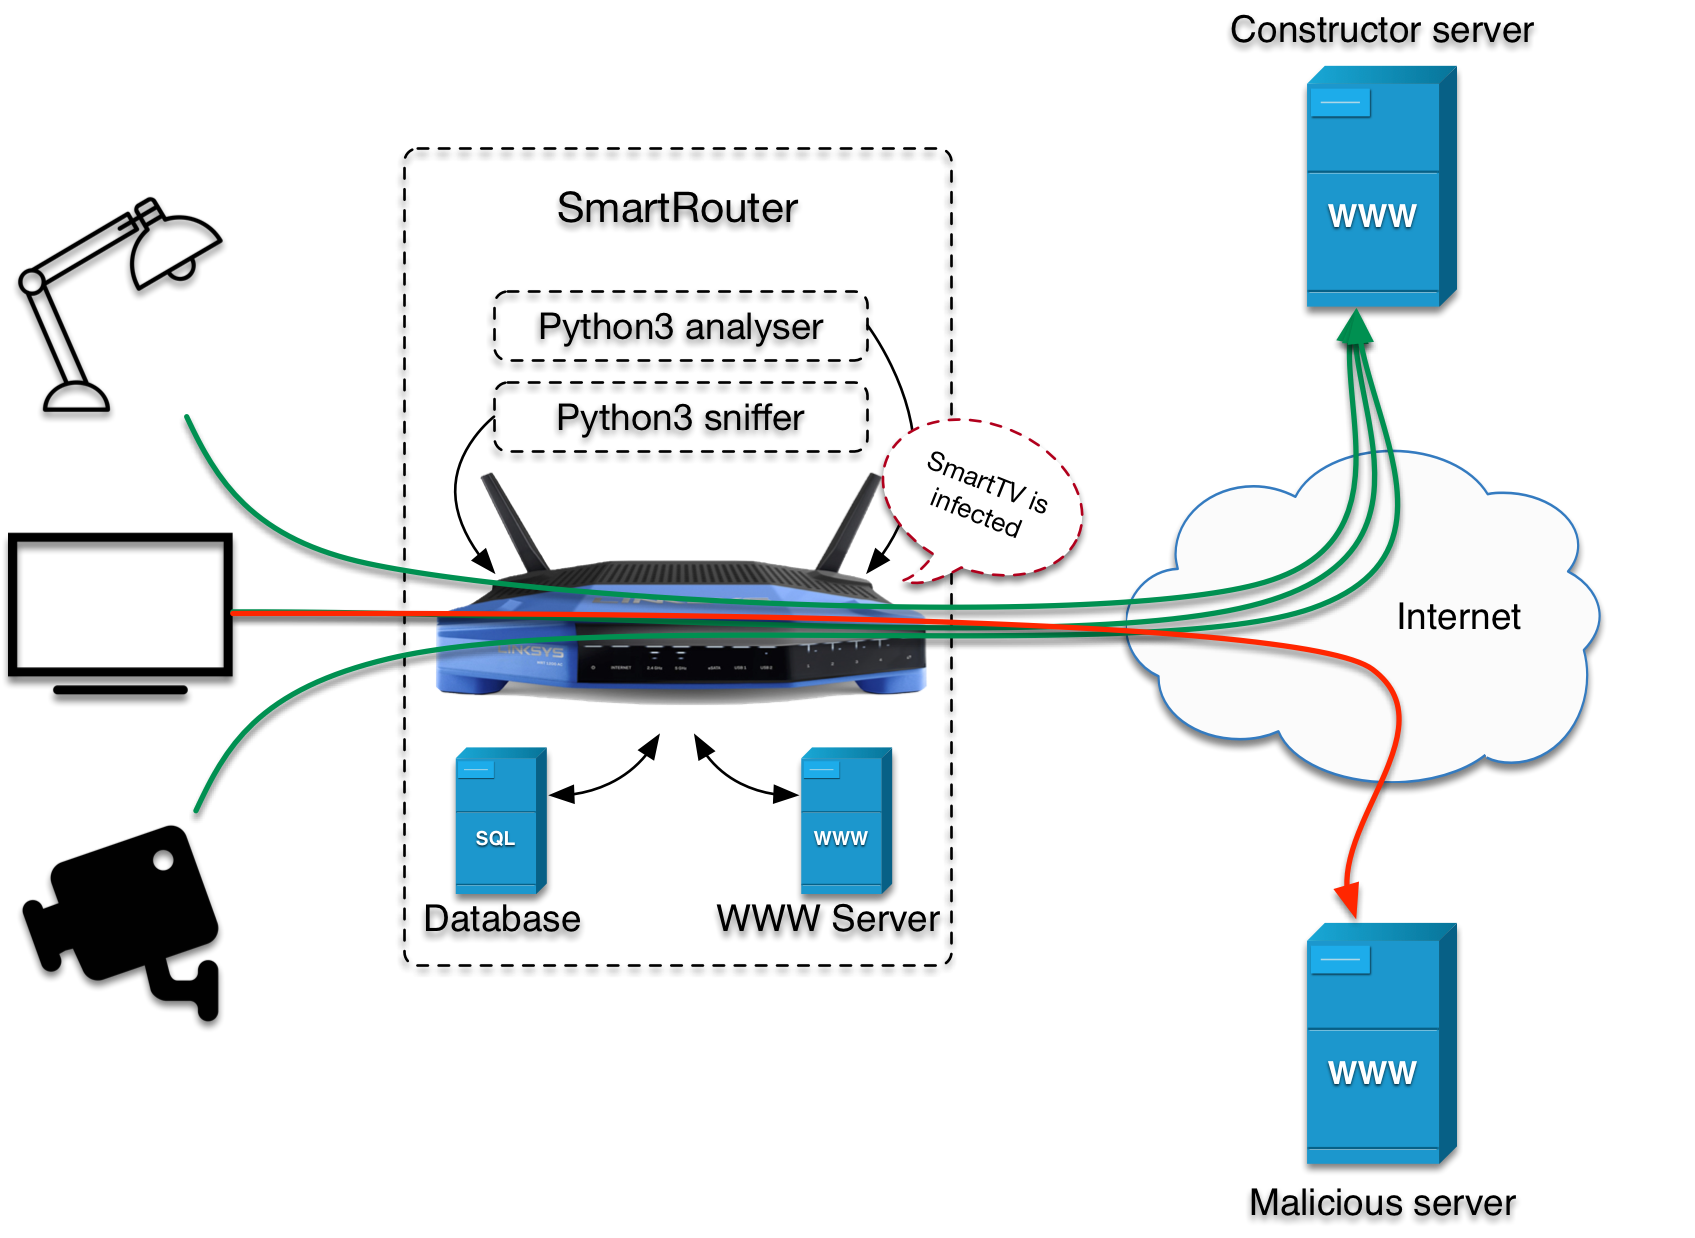
\includegraphics[width=\linewidth]{Pictures/design.png}


\subsection{Traffic sniffer}

The traffic sniffer is a process that captures all SYN packets with destination port TCP/80 \&\& TCP/443. This allows to detect all connection tentatives from the devices on the local network. For each tentative, following fields are stored in the database:

\begin{itemize}
\item Source MAC address,
\item Destination IP address,
\item Timestamp of the request
\end{itemize}

To be able to know to which domain corresponds each destination IP, DNS packets are also sniffed and then data are correlated to make IP correspond to a domain. If no domain corresponds to an IP, IPs are reversed lookup to try to have a domain.

Schematically, the process is the following : 
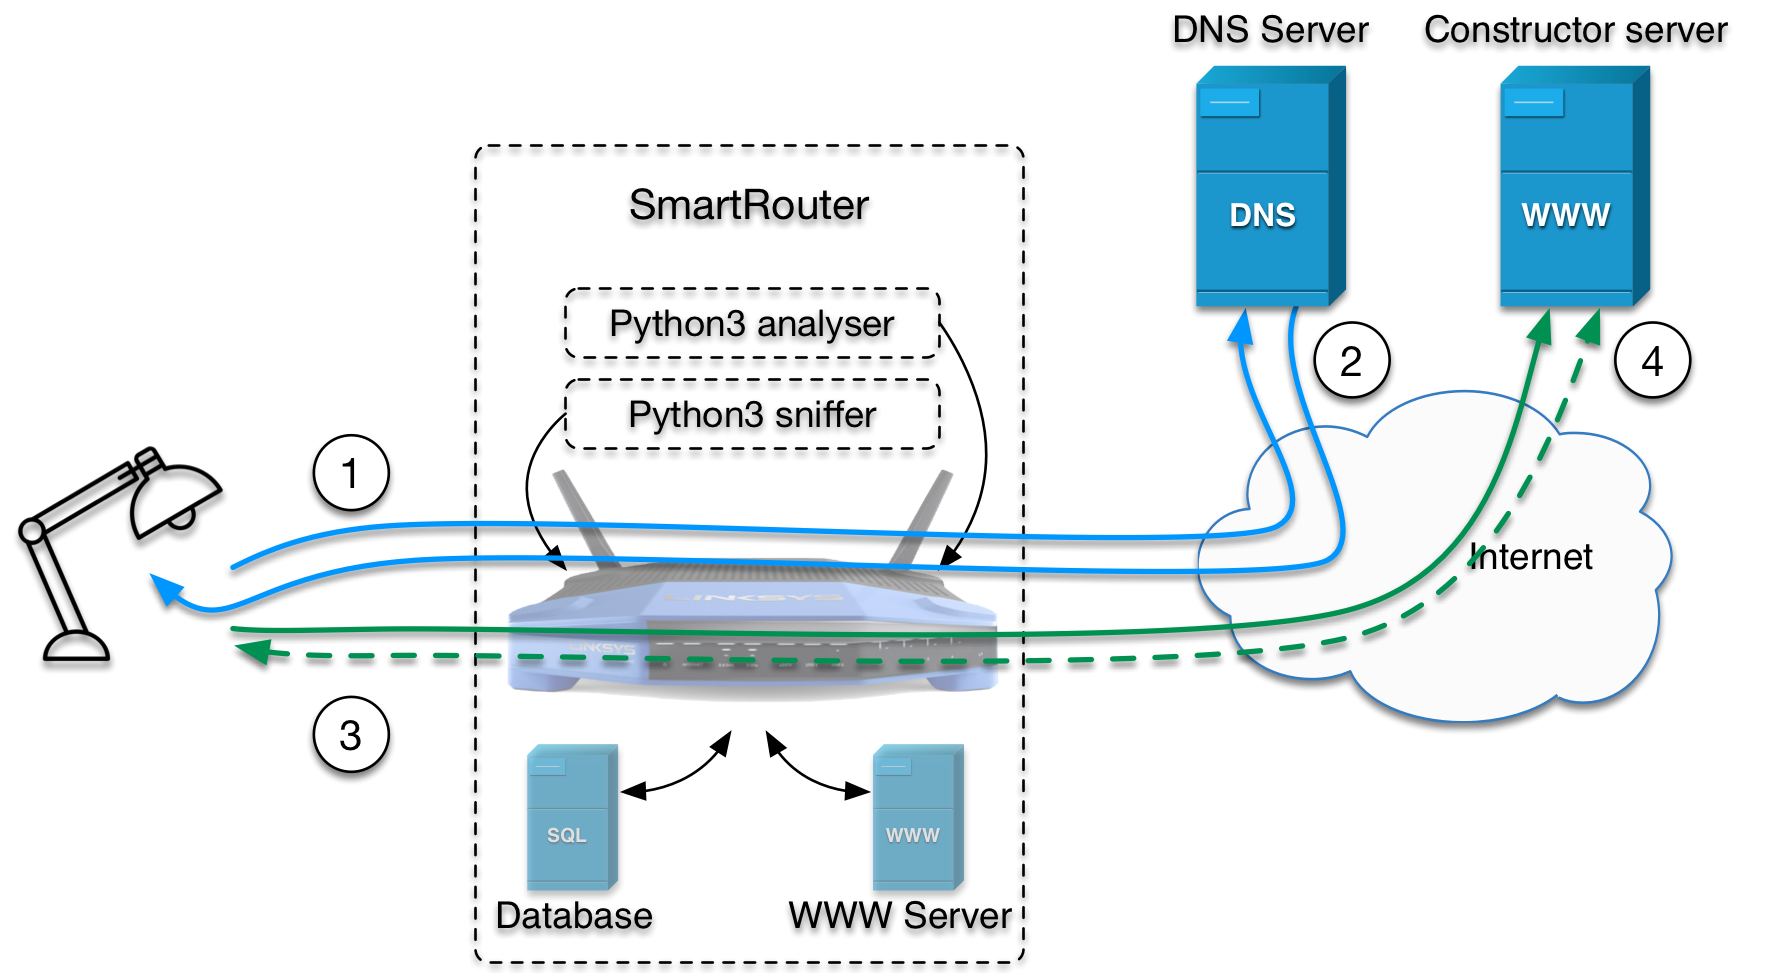
\includegraphics[width=\linewidth]{Pictures/dns.png}

\begin{enumerate}
\item First, the IoT sent a QNS query to \textit{constuctor.com} (assuming that this domain is the domain used for the IoT management, and which, in this case is legit). 
\item Second, the DNS server will reply to the previous request with the corresponding IP address of the previously asked domain. This request is sniffed, the domain and corresponding IP address are stored in the database
\item Third, the IoT will contact the server behind the previously asked domain. Only the SYN packet will be sniffed and an entry will be created into the database,
\item Finally, the rest of the request (non only SYN packets) will not be store into the database.
\end{enumerate}


\subsection{Traffic analyzer}

A process is launched every X minutes (depending of the setup) to analyze all traffic and determine if the traffic is legit or malicious. This process is managed by a custom \textit{init.d} script which is run at startup. \\


A "learning period" (which depend on the setup) is defined. Between the first request of an IoT and the end of the learning period, each packet and domains are considered as legit. \\


Beyond the period, if an IoT contact an unknown domain (which is a domain not contacted in the learning period), it will be considered like malicious. Is this case an alert will be generated and stored in the database.



Moreover, additional modules may be triggered when an alert occurs, like a Slack notification (see below), a notification on a dedicated app, a webhook etc.

\subsection{Web interface}
Actually the web interface displays only a txt file containing alerts. An example of truncated alert file id the following : 
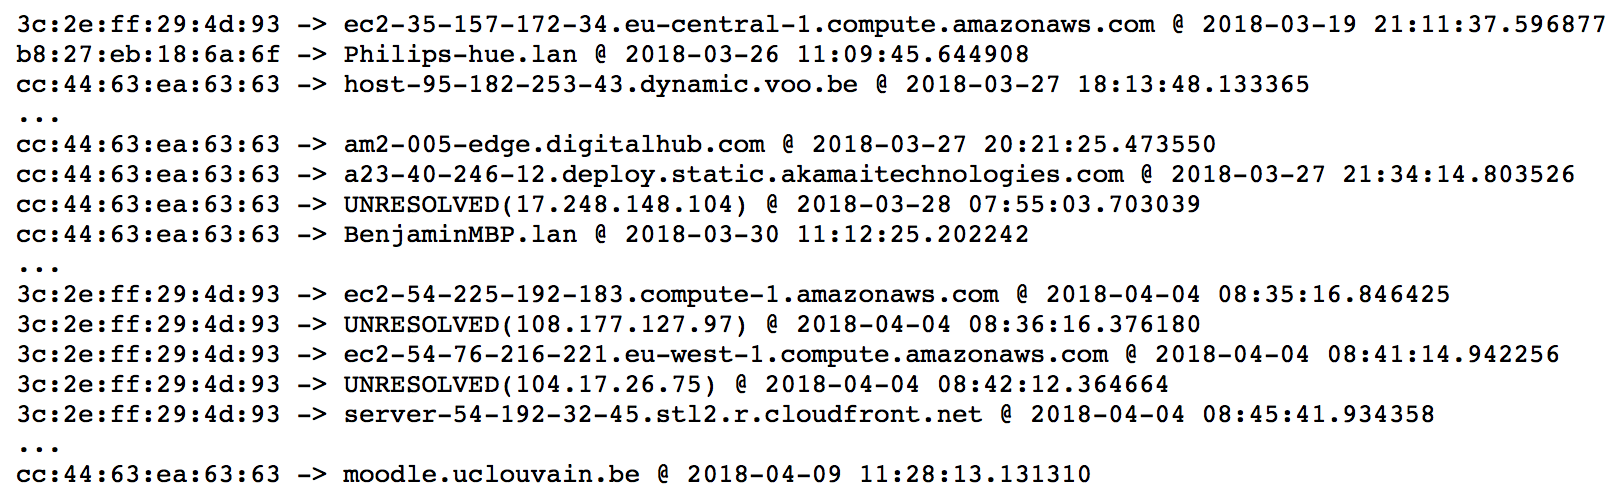
\includegraphics[width=\linewidth]{Pictures/alerts.png}

In the next version of this project, a web interface could be used to configure the router and have a better view of the alerts.


%\section{Tools}

\section{Implementation}

To test the detection system, we built a complete implementation, using OpenWRT, Python and Scapy.

The complete source code of the smart router is available at \url{https://github.com/RUCD/smart-router/}.

\subsection{OpenWRT $^{(\text{\url{https://openwrt.org}})}$}\\
The OpenWrt Project is a Linux operating system targeting embedded devices. So it was one of the possible choices for the Linux distribution. More specifically, OpenWRT was a compatible distribution for the router used for this project. The routers used are Linksys WRT1200ac.

\subsection{Scapy}\\

We used python and scapy to implement the traffic sniffer and the traffic analyzer. 
\textit{Scapy is a packet manipulation tool for computer networks, written in Python by Philippe Biondi. It can forge or decode packets, send them on the wire, capture them, and match requests and replies.}

%The main goal of the project is to have a router which executes 2 main tasks :
%\begin{itemize}
%  \item Sniff :  
%  \item Analyze : after having sniffed packet, 
%\end{itemize}

\subsection{Web server}\\
Due to portability issues and high resource consumption, we implemented a very simple web interface on the OpenWRT router: alerts are simply read on a text file and displayed vie a simple web server.


%\section{Installation}
%The installation is very simple thanks to auto-deploy scripts. A Readme is present to the Github the guide the installation. 

%Like routers used for this project do not have a lot of storage, a USB stick is needed to expand data storage. All this procedure is also explained in the Github(\url{https://github.com/RUCD/smart-router}).

%One of the auto-deploy script is the following :

%sh -c "\$(curl -fsSL https://raw.githubusercontent.com/\\
%RUCD/smart-router/master/docs/setupScripts/setupSR.sh)"


\section{Testing}
%Initially, two different types of alerting had been designed. On via a web browser, and another one, optional, like an application or something like that. 

We tested the smart router in various real SoHo networks. To be able to easily collect the alerts produced by the different routers, we implemented a slack application. This is a simple slack integration working with tokens. All is implemented by slack.

Slack alert have the role of the initial application alert. A slack application has been integrated in a workspace. So with it, the Smart Router send alert to a specific channel, thanks to slack tokens. 

This slack integration allow the receive notification like initially wanted, but without having to develop a specific application for it.

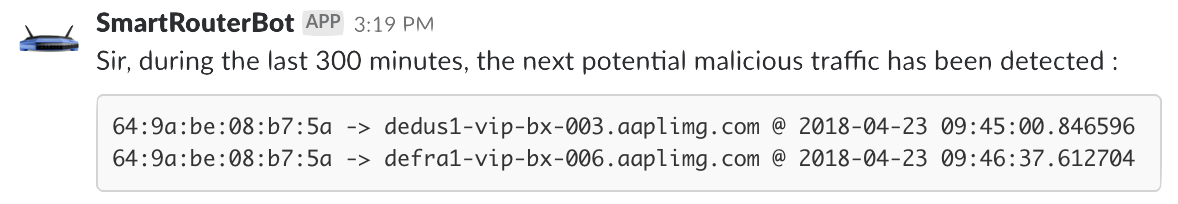
\includegraphics[width=\linewidth]{Pictures/slack.png}

\section{Future Work}
Lots of modules can be developed in future work, for example we can imagine : 
\begin{itemize}
	\item More protocol sniffed : for now, only web and DNS traffic is sniffed, but it could be interesting to have a generic sniffer which allowed to sniff everything traffic,
	
	\item Web configurations : all configuration is done in command line, so a more user-friendly web interface configuration page could be a great idea,
	
	\item Target sniffing : a good idea will be to be able to detect IoTs and filter only this traffic. Actually, all traffic is sniffed, but some can be blacklisted not to be sniffed,

	\item Target analysis : actually, all traffic is reanalyzed every time an analysis is run. A better analysis will be to analyze only new traffic since the last analysis,

	\item Lots of other integration are possible to have better interfaces and configuration modules.
\end{itemize}
% more protocols sniffed
% web server 


\section{Conclusion}
This project has a lot of other possibilities then experimented here. It also has a lot of optimization and machine learning possible. 

\end{multicols}
\end{frame}
\end{document}












